\documentclass[conference]{IEEEtran}
\IEEEoverridecommandlockouts
\usepackage{tikz}
\usetikzlibrary{shapes.geometric, arrows}
\usepackage{cite}
\usepackage{amsmath,amssymb,amsfonts}
\usepackage{algorithm}
\usepackage{algpseudocode}
\usepackage{graphicx}
\usepackage{textcomp}
\usepackage{xcolor}
\usepackage{pgfplots}
\usepackage{subfigure}

\pgfplotsset{compat=1.9}

\pgfplotsset{
    % #1: index in the group(0,1,2,...)
    % #2: number of plots of that group
    bar group size/.style 2 args={
        /pgf/bar shift={%
                % total width = n*w + (n-1)*skip
                % -> subtract half for centering
                -0.5*(#2*\pgfplotbarwidth + (#2-1)*\pgfkeysvalueof{/pgfplots/bar group skip})  + 
                % the '0.5*w' is for centering
                (.5+#1)*\pgfplotbarwidth + #1*\pgfkeysvalueof{/pgfplots/bar group skip}},%
    },
    bar group skip/.initial=2pt,
    plot 0/.style={blue,fill=blue!30!white,mark=none},%
    plot 1/.style={red,fill=red!30!white,mark=none},%
    plot 2/.style={brown!60!black,fill=brown!30!white,mark=none},%
    plot 3/.style={brown!60!black,fill=brown!30!white,mark=none},%
}

\def\BibTeX{{\rm B\kern-.05em{\sc i\kern-.025em b}\kern-.08em
    T\kern-.1667em\lower.7ex\hbox{E}\kern-.125emX}}

\makeatletter
\newcommand\fs@norules{\def\@fs@cfont{\bfseries}\let\@fs@capt\floatc@ruled
    \def\@fs@pre{}%
    \def\@fs@post{}%
    \def\@fs@mid{\kern3pt}%
    \let\@fs@iftopcapt\iftrue}
\makeatother

\tikzstyle{startstop} = [ellipse,minimum width=2cm, minimum height=1cm, text centered, draw=black, fill=white]
\tikzstyle{io} = [trapezium, trapezium left angle=70, trapezium right angle=110, minimum width=2cm, minimum height=1cm, text centered, draw=black, fill=white]
\tikzstyle{process} = [rectangle, minimum width=1cm, minimum height=1cm, text centered, draw=black, fill=white]
\tikzstyle{decision} = [diamond, minimum width=2cm, minimum height=1cm, text centered, draw=black, fill=white]
\tikzstyle{arrow} = [thick,->,>=stealth]

\newcommand\T{\rule{0pt}{2.6ex}}       % Top strut
\newcommand\B{\rule[-1.2ex]{0pt}{0pt}} % Bottom strut

\begin{document}

%%%%%%%%%%%%%%%%%%%%%%%%%%%%%%%%%%%%%%%%%%%%%%%%%%%%%%%%%%%%%%%%%%%%%%%%%%%%%%%%%%%
%%%%%%%%%%%%%%%%%%%%%%%%%%%%%%%%%%%%%% TITLE %%%%%%%%%%%%%%%%%%%%%%%%%%%%%%%%%%%%%%
%%%%%%%%%%%%%%%%%%%%%%%%%%%%%%%%%%%%%%%%%%%%%%%%%%%%%%%%%%%%%%%%%%%%%%%%%%%%%%%%%%%

\title{Improved Global Routing Using A-Star Algorithm\\}

%%%%%%%%%%%%%%%%%%%%%%%%%%%%%%%%%%%%%%%%%%%%%%%%%%%%%%%%%%%%%%%%%%%%%%%%%%%%%%%%%%%
%%%%%%%%%%%%%%%%%%%%%%%%%%%%%%%%%%%%% AUTHORS %%%%%%%%%%%%%%%%%%%%%%%%%%%%%%%%%%%%%
%%%%%%%%%%%%%%%%%%%%%%%%%%%%%%%%%%%%%%%%%%%%%%%%%%%%%%%%%%%%%%%%%%%%%%%%%%%%%%%%%%%

\author{\IEEEauthorblockN{AbdElrahman Elshafei\IEEEauthorrefmark{1}, Hossam Ahmed\IEEEauthorrefmark{2}, Mahmoud Mohamed\IEEEauthorrefmark{3} and Muhanad Atef\IEEEauthorrefmark{4}}
\IEEEauthorblockA{Computer Engineering Dept.,
Faculty of Engineering, Cairo University\\
Cairo, Egypt\\
\IEEEauthorrefmark{1}abdelrahman.elshafei98@gmail.com,
\IEEEauthorrefmark{2}hossamahmed201515@gmail.com,
\IEEEauthorrefmark{3}mmmacmp@gmail.com,
\IEEEauthorrefmark{4}muhanad.atef23@gmail.com}}


\maketitle

%%%%%%%%%%%%%%%%%%%%%%%%%%%%%%%%%%%%%%%%%%%%%%%%%%%%%%%%%%%%%%%%%%%%%%%%%%%%%%%%%%%
%%%%%%%%%%%%%%%%%%%%%%%%%%%%%%%%%%%% ABSTRACT %%%%%%%%%%%%%%%%%%%%%%%%%%%%%%%%%%%%%
%%%%%%%%%%%%%%%%%%%%%%%%%%%%%%%%%%%%%%%%%%%%%%%%%%%%%%%%%%%%%%%%%%%%%%%%%%%%%%%%%%%

\begin{abstract}
    In this paper we want to improve routing by improving global routing, this can be done by using A-Star algorithm, which will reduce time taken in this process and achieve the minimum wire length, many comparisons are taken in this paper with different algorithms to find the optimum algorithm to be used to achieve both minimum wire length and minimum time taken. From the comparisons of the paper we can find that using any algorithm is a trade off as when we decrease time taken, the wire length is increased and vice versa, so we cannot find an algorithm which is better from the other algorithms in general but we can say that using A-Star algorithm is a good approach to be used in global routing as it decreases the routing time however it is not the the best achieveable time but it is better than many other algorithms, and it is the best algorithm to achieve the minimum wire length with this complexity.
\end{abstract}

%%%%%%%%%%%%%%%%%%%%%%%%%%%%%%%%%%%%%%%%%%%%%%%%%%%%%%%%%%%%%%%%%%%%%%%%%%%%%%%%%%%
%%%%%%%%%%%%%%%%%%%%%%%%%%%%%%%%%%%% KEY WORDS %%%%%%%%%%%%%%%%%%%%%%%%%%%%%%%%%%%%
%%%%%%%%%%%%%%%%%%%%%%%%%%%%%%%%%%%%%%%%%%%%%%%%%%%%%%%%%%%%%%%%%%%%%%%%%%%%%%%%%%%

\begin{IEEEkeywords}
VLSI Routing, Global Routing, Routing Algorithms, Fast Global Routing, Fast Routing Algorithms, Routing Algoritms Comparisons.
\end{IEEEkeywords}

%%%%%%%%%%%%%%%%%%%%%%%%%%%%%%%%%%%%%%%%%%%%%%%%%%%%%%%%%%%%%%%%%%%%%%%%%%%%%%%%%%%
%%%%%%%%%%%%%%%%%%%%%%%%%%%%%%%%%% INTRODUCTION %%%%%%%%%%%%%%%%%%%%%%%%%%%%%%%%%%%
%%%%%%%%%%%%%%%%%%%%%%%%%%%%%%%%%%%%%%%%%%%%%%%%%%%%%%%%%%%%%%%%%%%%%%%%%%%%%%%%%%%

\section{Introduction}

Routing is critical step in physical design process. Until now the optimum solution for VLSI routing has not been achieved yet, so it is considered as a very interesting challenging feild. It is exactly done in two steps, global routing and detailed routing. At first global routing is run which is the responsible for making an approximate routing for the whole circuit in order to be used as a guide for detailed routing, then the detailed routing is run to make the exact routing for the system. That means if global or detailed routing is improved the whole routing process is improved, but there are many problems we have to overcome to make a correct routing process. First of all we have to take into consideration the scale, as millions of wires exist in a small chip area which means that many kilometers of wires are placed in a very small area, so we have to minimize total wire length as much as we can, also we know that as the wire length increases the resistance increases as well which means more delay in the chip. We can find another problem as circuits are made in nano-scale which means that its geometric will be complex. Another problem that routing algorithm have to be applicable for more than one layer with different costs. We also have to take into consideration the direction of wires in every layer (vertical | horizontal) and no diagonal pathes, then to go from source 'S' to target 'T' the path taken should be in (vertical | horizontal) directions thet specified by the layer (at each layer wires are placed in one direction only), then there is another problem as when a wire goes from layer to another to continue on the perpendicular direction it have to go through via which have a high resistance. DFM (design for manufacturer) rules also has to be achieved. All of these constraints must be taken into consideration with the global routing to achieve hundred percent of the circuit connections, that means global routing will take a lot of time to achieve all these constraints, and here is the challenge to achieve all the routing specifications with minimum time taken. 

\begin{figure} 
\centering  
\subfigure[First iteration] {
    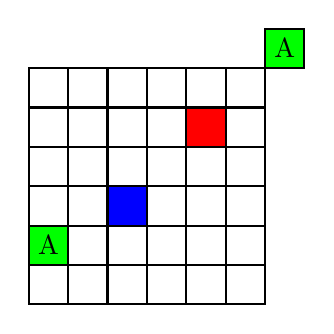
\begin{tikzpicture}
        [
            box/.style={rectangle,draw=black,thick, minimum size=0.5cm},
        ]
    
    \foreach \x in {0,0.5,...,2.5}{
        \foreach \y in {0,0.5,...,2.5}
            \node[box] at (\x,\y){};
    }
    \node [box,fill=green] at (0,0.5){A};  
    \node[box,fill=green] at (3,3){A};  
    \node[box,fill=red  ] at (2,2){};  
    \node[box,fill=blue ] at (1,1){};  
    \end{tikzpicture}
}
\subfigure[Second iteration] {
    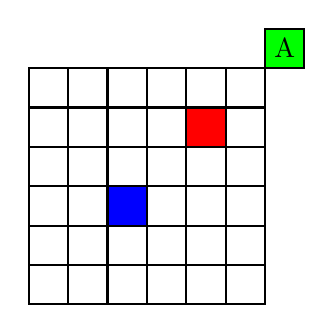
\begin{tikzpicture}
        [
            box/.style={rectangle,draw=black,thick, minimum size=0.5cm},
        ]
    
    \foreach \x in {0,0.5,...,2.5}{
        \foreach \y in {0,0.5,...,2.5}
            \node[box] at (\x,\y){};
    }
    
    \node[box,fill=green] at (3,3){A};  
    \node[box,fill=red  ] at (2,2){};  
    \node[box,fill=blue ] at (1,1){};  
    \end{tikzpicture}
}
\subfigure[Third iteration] {
    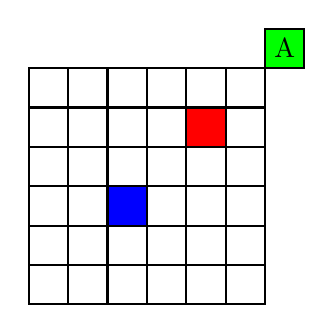
\begin{tikzpicture}
        [
            box/.style={rectangle,draw=black,thick, minimum size=0.5cm},
        ]
    
    \foreach \x in {0,0.5,...,2.5}{
        \foreach \y in {0,0.5,...,2.5}
            \node[box] at (\x,\y){};
    }
    
    \node[box,fill=green] at (3,3){A};  
    \node[box,fill=red  ] at (2,2){};  
    \node[box,fill=blue ] at (1,1){};  
    \end{tikzpicture}
}
\subfigure[After N iteration] {
    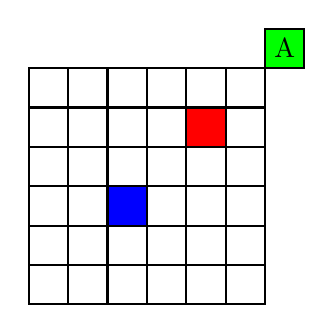
\begin{tikzpicture}
        [
            box/.style={rectangle,draw=black,thick, minimum size=0.5cm},
        ]
    
    \foreach \x in {0,0.5,...,2.5}{
        \foreach \y in {0,0.5,...,2.5}
            \node[box] at (\x,\y){};
    }
    
    \node[box,fill=green] at (3,3){A};  
    \node[box,fill=red  ] at (2,2){};  
    \node[box,fill=blue ] at (1,1){};  
    \end{tikzpicture}
}
\caption{Steps to get the best global routing}
\label{fig:GlobalRoutingProcess}
\end{figure}

In Figure~\ref{fig:GlobalRoutingProcess} 


%%%%%%%%%%%%%%%%%%%%%%%%%%%%%%%%%%%%%%%%%%%%%%%%%%%%%%%%%%%%%%%%%%%%%%%%%%%%%%%%%%%
%%%%%%%%%%%%%%%%%%%%%%%%%%%%%%%%%% RELATED WORK %%%%%%%%%%%%%%%%%%%%%%%%%%%%%%%%%%%
%%%%%%%%%%%%%%%%%%%%%%%%%%%%%%%%%%%%%%%%%%%%%%%%%%%%%%%%%%%%%%%%%%%%%%%%%%%%%%%%%%%

\section{Related Work}

Several papers proposed various types of approaches to improve the overall efficiency of the multilevel feedback queue scheduling algorithm. The chosen quantum time for each queue plays a major role. Hence, it is essential to choose a proper method to compute the time quantum value to minimize response time and maximize overall performance. In , an algorithm is introduced for minimizing the response time. In this algorithm, a Recurrent Neural Network (RNN) is used to determine both the number of queues and the optimized time quantum value for each queue. The RNN generates an effective model to compute the time quantum value. Their proposed intelligent version of the MLFQ offers good results, however, it suffers from a few drawbacks, the first being the direct proportionality of its network learning time and the amount of input data, and the second is the possibility of experiencing initial overhead at the first iterations of the algorithm. Our approach proposes an improved version of MLFQ that utilizes an altered version of RR named shortest remaining burst round-robin (SRBRR) introduced in  which avoids the cost of learning time and overhead time in . Regarding the various approaches to improve the MLFQ algorithm, those attempts dealt with starvation by assigning different quantum values to the ready queues depending on their priority. Our approach also deals with starvation by boosting processes from lower priority queues to higher ones according to certain criteria.

%%%%%%%%%%%%%%%%%%%%%%%%%%%%%%%%%%%%%%%%%%%%%%%%%%%%%%%%%%%%%%%%%%%%%%%%%%%%%%%%%%%
%%%%%%%%%%%%%%%%%%%%%%%%%%%%%%%% PROPOSED APPROACH %%%%%%%%%%%%%%%%%%%%%%%%%%%%%%%%
%%%%%%%%%%%%%%%%%%%%%%%%%%%%%%%%%%%%%%%%%%%%%%%%%%%%%%%%%%%%%%%%%%%%%%%%%%%%%%%%%%%

\section{Proposed Approach}

For a multilevel feedback queue scheduling algorithm, three parameters are considered. The first is the chosen scheduling algorithm for each queue, especially the last queue as its scheduling algorithm is expected to treat starvation. The second is the criteria according to which a process is promoted, this technique is also known as Aging. The third is the criteria according to which a process is demoted. In our proposed algorithm, there are 5 queues sorted in ascending order in line with their priority number, 1 being the highest priority and 5 being the lowest. Each queue uses a modified version of the round-robin scheduling algorithm stated in {b3}. In {b3}, processes are sorted in ascending order according to their burst time and are assigned a time quantum that equals the median burst time of those processes. This algorithm provides better turnaround time and waiting time than the standard static quantum RR algorithm whose quantum, if set too short, leads to many context switches and, if set too long, morphs the algorithm into an FCFS algorithm. The proposed alteration on the stated algorithm in {b3} is that each queue quantum time equals the median burst time multiplied by a factor matching the queue number. Hence, the gradual increase of quantum time as priority decreases. For clarification, a queue with priority equal $2$ has the following processes denoted by their burst time: $100$, $300$, $550$, $600$, $620$, $700$, $720$, $900$ and $1200$, the median value is $620$, since we are in a queue whose priority equals $2$, therefore the quantum slice value according to the proposed approach equals $1240$ as in $620 * 2$. If processes of a certain queue didn't terminate after assigning the quantum time value, they are shifted to the next lower priority queue. After introducing new processes into a queue, the quantum time slice is recalculated. Processes age whenever they are in a queue whose priority is one less than that currently getting scheduled and satisfies the following inequality:
\begin{equation}
\frac{waiting \; time \; of \; P}{burst \; time \; of \; P} >= 1\label{eq1}
\end{equation}

Those procedures are repeated for all the generated queues until all processes reach the lowest priority queue where they are rescheduled until their completion. 

%%%%%%%%%%%%%%%%%%%%%%%%%%%%%%%%%%%%%%%%%%%%%%%%%%%%%%%%%%%%%%%%%%%%%%%%%%%%%%%%%%%
%%%%%%%%%%%%%%%%%%%%%%%%%%%%%%%%%%%% FLOWCHART %%%%%%%%%%%%%%%%%%%%%%%%%%%%%%%%%%%%
%%%%%%%%%%%%%%%%%%%%%%%%%%%%%%%%%%%%%%%%%%%%%%%%%%%%%%%%%%%%%%%%%%%%%%%%%%%%%%%%%%%

\subsection{Pseudocode Flowchart of the Proposed Approach}
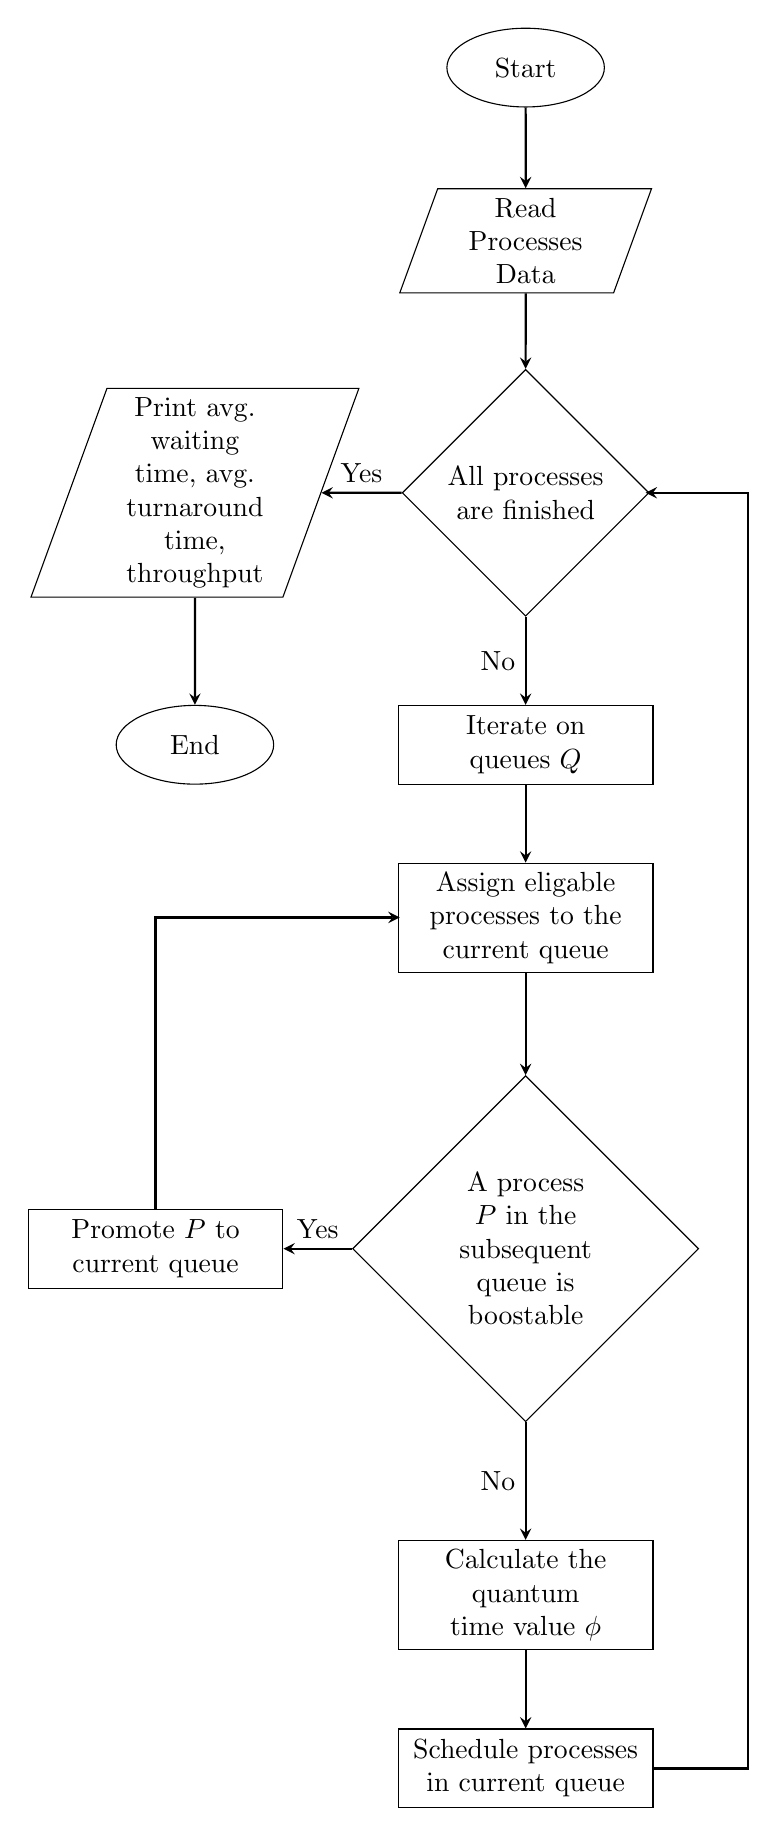
\begin{tikzpicture}[node distance=2.2cm]

    \node (start) [startstop] {Start};
    \node (in1) [io, below of=start, text width = 2cm] {Read Processes Data};
    \node (dec1) [decision, below of=in1, text width = 2cm, yshift=-1cm] {All processes are finished};
    \node (pro1) [process, below of=dec1, text width= 3cm, yshift = -1cm] {Iterate on queues $Q$};
    \node (pro2) [process, below of=pro1, text width = 3cm] {Assign eligable processes to the current queue};
    \node (out1) [io, left of=dec1, text width = 2cm, xshift= -2cm] {Print avg. waiting time, avg. turnaround time, throughput};
    \node (end) [startstop, below of=out1, yshift=-1cm] {End};
    \node (dec2) [decision, below of=pro2, text width = 2cm, yshift=-2cm] {A process $P$ in the subsequent queue is boostable};

    \node (pro3) [process, left of=dec2, text width= 3cm, xshift= -2.5cm] {Promote $P$ to current queue};
    \node (pro4) [process, below of=dec2, text width= 3cm, yshift=-2.2cm] {Calculate the quantum time value $\phi$};
    \node (pro5) [process, below of=pro4, text width= 3cm] {Schedule processes in current queue};
    
    \draw [arrow] (start) -- (in1);
    \draw [arrow] (in1) -- (dec1);
    % \draw [arrow] (pro1) -- (dec1);
    \draw [arrow] (dec1) -- node[anchor=west, above] {Yes} (out1);
    \draw [arrow] (out1) -- (end);
    \draw [arrow] (dec1) -- node[anchor=south, left] {No} (pro1);
    \draw [arrow] (pro1) -- (pro2);
    \draw [arrow] (pro2) -- (dec2);
    \draw [arrow] (dec2) -- node[anchor=west,above] {Yes} (pro3);
    \draw [arrow] (pro3.north) -- ++ (0,3.7) -- ++ (3.1,0);
    \draw [arrow] (dec2) -- node[anchor=south, left] {No} (pro4);
    \draw [arrow] (pro4) -- (pro5);
    \draw [arrow] (pro5.east) -- ++ (1.2,0) -- ++(0,16.2) -- ++(-1.3,0);
    \end{tikzpicture}

%%%%%%%%%%%%%%%%%%%%%%%%%%%%%%%%%%%%%%%%%%%%%%%%%%%%%%%%%%%%%%%%%%%%%%%%%%%%%%%%%%%
%%%%%%%%%%%%%%%%%%%%%%%%%%%%%%%%%%%% ALGORITHM %%%%%%%%%%%%%%%%%%%%%%%%%%%%%%%%%%%%
%%%%%%%%%%%%%%%%%%%%%%%%%%%%%%%%%%%%%%%%%%%%%%%%%%%%%%%%%%%%%%%%%%%%%%%%%%%%%%%%%%%

\subsection{Proposed Algorithm}
% \floatstyle{norules}
\restylefloat{algorithm}
\begin{algorithm}[H]
    \caption{Developed Multilevel Feedback Queue Scheduling Algorithm}
    \hspace*{\algorithmicindent} \textbf{Input:} Number of processes $n$, processes priority $\alpha$\\
    \hspace*{\algorithmicindent} burst time values $\beta$, arrival time values $\sigma$, \\
    \hspace*{\algorithmicindent} context switching cost $\epsilon$\\
    \hspace*{\algorithmicindent} \textbf{Output:} Average turnaround time, average waiting time,\\
    \hspace*{\algorithmicindent} throughput
    \begin{algorithmic}[1]
    \Procedure {DMLFQ}{}
    % Return  Average waiting time, throughput
    \Statex Declaration and Initialisation:
    \State Queue $Q_{i}$ where $i \in \{1, 2, 3, 4, 5\}$
    \State Turnaround time values $\tau$
    \State Finish time values $\lambda$
    \State Waiting time values $\theta$
    \State Remaining time values $\mu = \beta$
    \State Quantum time value $\phi$
    \State Number of context switches $\delta$
        \State$time = 0$
        \While{$\exists P \in Q$}
            \For{$i = 1$ to $5$}
                \For{$j = 1$ to $n$}
                    \If{$\sigma_{j} <= time$ and $\alpha_{j}$ equals $i$}
                        \State \textit{\textbf{Assign}} $P_{j}$ to $Q_{i}$
                    \EndIf
                    \State $waitingTime = time - \sigma_{j}$
                    \If{$i < 5$ and $waitingTime/\mu_{j} >= 1$ and $\alpha_{j}$ equals $i + 1$ and  $\sigma_{j} <= time$}
                        \State \textit{\textbf{Assign}} $P_{j}$ to $Q_{i}$
                    \EndIf
                \EndFor
                \State Sort $Q_{i}$ in ascending order according to remaining time values
                \State $\phi = median\; value\; of\; Q_{i} * i$
                \algrenewcommand\algorithmicfor{\textbf{foreach}}
                \For{$P_{j} \in Q_{i}$}
                    \If{$\mu_{j} <= \phi$}
                        \State $time = time + \mu_{j}$
                        \State $\lambda_{j} = time$
                        \State \textit{\textbf{Remove}} $P_{j}$ from $Q_{i}$
                    \Else
                        \State $time = time + \phi$
                        \State $\mu_{j} = \mu_{j} - \phi$
                        \If{$i < 5$}
                            \State $\alpha_{j} = \alpha_{j} + 1$
                        \EndIf
                    \EndIf
                    \If{Previous process $\neq P_{j}$}
                        \State $time = time + \epsilon$
                        \State $\delta = \delta + 1$
                    \EndIf
                \EndFor
                \algrenewcommand\algorithmicfor{\textbf{for}}
            \EndFor
        \EndWhile
        \For{$i = 1$ to $n$}
            $\tau_{j} = \lambda_{j} - \sigma_{j}$, $\theta_{j} = \tau_{j} - \beta_{j}$
        \EndFor
        \State \textbf{return} average of $\theta$, average of $\tau$, $n/time$
        \EndProcedure
    \end{algorithmic}
\end{algorithm}

%%%%%%%%%%%%%%%%%%%%%%%%%%%%%%%%%%%%%%%%%%%%%%%%%%%%%%%%%%%%%%%%%%%%%%%%%%%%%%%%%%%
%%%%%%%%%%%%%%%%%%%%%%%%%%%%%% EXPERIMENTAL ANALYSIS %%%%%%%%%%%%%%%%%%%%%%%%%%%%%%
%%%%%%%%%%%%%%%%%%%%%%%%%%%%%%%%%%%%%%%%%%%%%%%%%%%%%%%%%%%%%%%%%%%%%%%%%%%%%%%%%%%

\section{Experimental Analysis}

%%%%%%%%%%%%%%%%%%%%%%%%%%%%%%%%%%%%%%%%%%%%%%%%%%%%%%%%%%%%%%%%%%%%%%%%%%%%%%%%%%%
%%%%%%%%%%%%%%%%%%%%%%%%%%%%%%%%%%% ASSUMPTIONS %%%%%%%%%%%%%%%%%%%%%%%%%%%%%%%%%%%
%%%%%%%%%%%%%%%%%%%%%%%%%%%%%%%%%%%%%%%%%%%%%%%%%%%%%%%%%%%%%%%%%%%%%%%%%%%%%%%%%%%

\subsection{Assumptions}

The proposed scheduling algorithm is software simulated using a Python script which simulates scheduling independent CPU-bound processes on a single processor environment which guarantees that no more than a single process is getting scheduled at any arbitrary moment. Each process is assumed to have its own predetermined burst time, arrival time and the queue to which each one belongs. The proposed approach is non-preemptive. For the sake of giving an example, if a process was lately introduced to a queue denoted by $Q_{i}$ prior to the current queue getting scheduled, it won't get scheduled until the current queue, its subsequent queues and the queues prior to $Q_{i}$ get scheduled.

%%%%%%%%%%%%%%%%%%%%%%%%%%%%%%%%%%%%%%%%%%%%%%%%%%%%%%%%%%%%%%%%%%%%%%%%%%%%%%%%%%%
%%%%%%%%%%%%%%%%%%%%%%%%%%%%%%%%%%%%%%% I/O %%%%%%%%%%%%%%%%%%%%%%%%%%%%%%%%%%%%%%%
%%%%%%%%%%%%%%%%%%%%%%%%%%%%%%%%%%%%%%%%%%%%%%%%%%%%%%%%%%%%%%%%%%%%%%%%%%%%%%%%%%%

\subsection{Experimental Scheme}

On one hand, the input arguments to the proposed algorithm implementation are the number of processes to be scheduled, their burst time, their arrival time and the queue where each one belongs. On the other hand, output parameters are the average waiting time, average turnaround time and throughput. The following equations are used to calculate the previously mentioned output parameters:

\begin{equation}
    Average\; Waiting\; Time =  \frac{Total \; Waiting \; Time}{Number \; of \; Processes} \label{eq2}
\end{equation}

\begin{equation}
    Average\; Turnaround\; Time =  \frac{Total \; Turnaround \; Time}{Number \; of \; Processes} \label{eq3}
\end{equation}

\begin{equation}
    Throughput =  \frac{Number \; of \; Executed \; Processes}{Total \; Execution \; Time} \label{eq4}
\end{equation}

% \vspace{4mm}

%%%%%%%%%%%%%%%%%%%%%%%%%%%%%%%%%%%%%%%%%%%%%%%%%%%%%%%%%%%%%%%%%%%%%%%%%%%%%%%%%%%
%%%%%%%%%%%%%%%%%%%%%%%%%%%%%%% PERFORMANCE METRICS %%%%%%%%%%%%%%%%%%%%%%%%%%%%%%%
%%%%%%%%%%%%%%%%%%%%%%%%%%%%%%%%%%%%%%%%%%%%%%%%%%%%%%%%%%%%%%%%%%%%%%%%%%%%%%%%%%%

\subsection{Performance Metrics}

As a means to have a concrete, viable evaluation of either the proposed algorithm or any other scheduling algorithm, the output parameters are taken into consideration for analysis. Since the average waiting time indicates the average time that a  process had to starve for, therefore the lower the average waiting time is the better. The same principle applies to the average turnaround time and the number of context switches, as the former implies the average time spent by the process since its arrival time to its completion and the latter costs time as the CPU is assigned back and forth between different processes. Contrarily to the prior metrics, the larger the throughput is the better as it indicates the number of processes that are completely executed per unit time.

%%%%%%%%%%%%%%%%%%%%%%%%%%%%%%%%%%%%%%%%%%%%%%%%%%%%%%%%%%%%%%%%%%%%%%%%%%%%%%%%%%%
%%%%%%%%%%%%%%%%%%%%%%%%%%%%%%%%%%% SIMULATION %%%%%%%%%%%%%%%%%%%%%%%%%%%%%%%%%%%%
%%%%%%%%%%%%%%%%%%%%%%%%%%%%%%%%%%%%%%%%%%%%%%%%%%%%%%%%%%%%%%%%%%%%%%%%%%%%%%%%%%%

\subsection{Simulation}

For the sake of showcasing the proposed algorithm, a number of processes, their predetermined burst time values and their arrival time values are taken as input to the Python simulation script. Suppose that the input to the script is according to the following table:

\begin{table}[H]
    \caption{}
    \centering
     \begin{tabular}{||c c c c||} 
     \hline
     \textit{\textbf{Process}} & \textit{\textbf{Arrival Time}} & \textit{\textbf{Burst Time}} & \textit{\textbf{Queue}} \T \B \\ 
     \hline
     \hline
     1 & 0 & 60 & 1 \T \B \\ 
     \hline
     2 & 0 & 50 & 1 \T \B \\
     \hline
     3 & 0 & 40 & 2 \T \B \\
     \hline
     4 & 0 & 30 & 2 \T \B \\
     \hline
     5 & 0 & 10 & 3 \T \B \\ 
     \hline
     6 & 0 & 210 & 3 \T \B \\ 
     \hline
     7 & 0 & 200 & 3 \T \B \\ 
     \hline
     \end{tabular}
     \label{table1}
\end{table}

According to the proposed algorithm, the time quanta calculated are as follows:

\begin{table}[H]
    \caption{}
    \centering
     \begin{tabular}{||c c||} 
     \hline
     \textit{\textbf{Queue}} & \textit{\textbf{Quantum Value}} \T \B \\ 
     \hline
     \hline
     1 & 55 \T \B \\ 
     \hline
     2 & 40 \T \B \\
     \hline
     3 & 615 \T \B \\
     \hline
     4 & 0 \T \B \\
     \hline
     5 & 0 \T \B \\ 
     \hline
     \end{tabular}
\end{table}

All processes are sorted in ascending order according to their remaining time and are scheduled by assigning the time quantum calculated for their respective queue. The time spent scheduling a particular queue is the waiting time for its subsequent queues.

The scheduling process goes as follows:

\begin{figure}[H]
        \begin{center}
        \begin{tabular}{|c|c|}
         \hline
            $P_{2}$ & $P_{1}$\T\B\\ 
         \hline
        \end{tabular}
        \end{center}
        \begin{center}
            \begin{tabular}{c c c}
                   0 & 50 & 105\\ 
            \end{tabular}
        \end{center}
    \caption{$Q_{1}$ Gantt Chart}
\end{figure}

Considering that each process in $Q_{1}$ is assigned a quantum value of $50$, as we reach the last process in $Q_{1}$, the total time elapsed equals $105$, which happens to be the time that all the other processes in the subsequent queues had to wait for, hence the addition of their waiting time by a value of $105$ units of time.

\begin{figure}[H]
    \begin{center}
    \begin{tabular}{|c|c|c|c|}
     \hline
        $P_{1}$ & $P_{5}$ & $P_{4}$ & $P_{3}$\T\B\\ 
     \hline
    \end{tabular}
    \end{center}
    \begin{center}
        \begin{tabular}{c c c c c}
               105 & 110 & 120 & 150 & 190\\ 
        \end{tabular}
    \end{center}
\caption{$Q_{2}$ Gantt Chart}
\end{figure}

Even though $P_{5}$ is initially assigned to $Q_{3}$ as in Table \ref{table1}, it was promoted to $Q_{2}$ due to satisfying inequality (\ref{eq1}).

\begin{figure}[H]
    \begin{center}
    \begin{tabular}{|c|c|}
     \hline
        P7 & P6\T\B\\ 
     \hline
    \end{tabular}
    \end{center}
    \begin{center}
        \begin{tabular}{c c c}
               190 & 390 & 600\\ 
        \end{tabular}
    \end{center}
\caption{$Q_{3}$ Gantt Chart}
\end{figure}

Whenever processes reach the lowest queue precompletion, they are scheduled using the RR scheduling algorithm with a relatively large quantum time value which is in most cases similar to using the FCFS algorithm because, as the time quantum value of an RR algorithm tends to infinity which could practically be a very large number relative to the available processes remaining time values, the algorithm tends to morph into the FCFS algorithm. This procedure is iterated until all the processes are finished. Simulation results are shown in the table below:

\begin{table}[H]
    \caption{}
    \centering
     \begin{tabular}{||c c c||} 
     \hline
     \textit{\textbf{Avg. Turnaround Time}} & \textit{\textbf{Avg. Waiting Time}} & \textit{\textbf{Throughput}}\T \B \\ 
     \hline
     \hline
     230 & 144.3 & 0.011667 \T \B \\ 
     \hline
     \end{tabular}
\end{table}

%%%%%%%%%%%%%%%%%%%%%%%%%%%%%%%%%%%%%%%%%%%%%%%%%%%%%%%%%%%%%%%%%%%%%%%%%%%%%%%%%%%
%%%%%%%%%%%%%%%%%%%%%%%%%%%%%%%%%%% COMPARISONS %%%%%%%%%%%%%%%%%%%%%%%%%%%%%%%%%%%
%%%%%%%%%%%%%%%%%%%%%%%%%%%%%%%%%%%%%%%%%%%%%%%%%%%%%%%%%%%%%%%%%%%%%%%%%%%%%%%%%%%

\subsection{Performance Comparisons}

To assess the performance of the proposed algorithm implementation, multiple test cases are addressed and analyzed in seven different experiments. In each experiment, the output of the proposed algorithm implementation is compared to the output of another scheduling algorithm implementation addressed in a different paper, such as standard MLFQ algorithm with static quantum RR and other variants of MLFQ algorithms and RR algorithms.

\subsubsection{Experiment 1}

In this experiment, the proposed algorithm is compared against two MLFQ algorithm variants stated in {b4}. The first uses a static version of the RR algorithm for scheduling each queue, while the second variant uses a dynamic version of the RR algorithm for doing so.

\begin{table}[H]
    \caption{Experiment 1 Input}
    \centering
     \begin{tabular}{||c c c c||} 
     \hline
     \textit{\textbf{Process}} & \textit{\textbf{Arrival Time}} & \textit{\textbf{Burst Time}} & \textit{\textbf{Queue}} \T \B \\ 
     \hline
     \hline
     1 & 1 & 25 & 1 \T \B \\ 
     \hline
     2 & 5 & 70 & 1 \T \B \\
     \hline
     3 & 6 & 84 & 1 \T \B \\
     \hline
     4 & 7 & 17 & 1 \T \B \\
     \hline
     5 & 8 & 35 & 1 \T \B \\ 
     \hline
     \end{tabular}
\end{table}

\begin{table}[H]
    \caption{Experiment 1 Results}
    \centering
    \begin{tabular}{||c c c||}
        \hline
        \textit{\textbf{Algorithm}} & \textit{\textbf{Avg. Turnaround Time}} & \textit{\textbf{Avg. Waiting Time}}\T \B \\
    \hline
    \hline
    \textbf{Proposed Algorithm} & 115 & 68.8 \T \B\\ \hline
    \textbf{Dynamic RR MLFQ} & 150.8 & 107.6\T \B\\ \hline
    \textbf{Static RR MLFQ} & 161.4 & 116.2 \T \B\\ \hline
     \end{tabular}
\end{table}

\subsubsection{Experiment 2}

In this experiment, the proposed algorithm is compared against two MLFQ algorithm variants stated in {b4}. The first uses a static version of the SJFRR algorithm for scheduling each queue, while the second variant uses a dynamic version of the SJFRR algorithm for doing so. 

\begin{table}[H]
    \caption{Experiment 2 Input}
    \centering
     \begin{tabular}{||c c c c||} 
     \hline
     \textit{\textbf{Process}} & \textit{\textbf{Arrival Time}} & \textit{\textbf{Burst Time}} & \textit{\textbf{Queue}} \T \B \\ 
     \hline
     \hline
     1 & 1 & 25 & 1 \T \B \\ 
     \hline
     2 & 5 & 70 & 1 \T \B \\
     \hline
     3 & 6 & 84 & 1 \T \B \\
     \hline
     4 & 7 & 17 & 1 \T \B \\
     \hline
     5 & 8 & 35 & 1 \T \B \\ 
     \hline
     \end{tabular}
\end{table}

\begin{table}[H]
    \caption{Experiment 2 Results}
    \centering
    \begin{tabular}{||c c c||}
        \hline
        \textit{\textbf{Algorithm}} & \textit{\textbf{Avg. Turnaround Time}} & \textit{\textbf{Avg. Waiting Time}}\T \B \\
    \hline
    \hline
    \textbf{Proposed Algorithm} & 115 & 68.8 \T \B\\ \hline
    \textbf{Dyn. SJFRR MLFQ} & 134 & 91.8\T \B\\ \hline
    \textbf{Stat. SJFRRMLFQ} & 143.4 & 98.2 \T \B\\ \hline
     \end{tabular}
\end{table}

\subsubsection{Experiment 3}

In this experiment, the proposed algorithm is compared against two MLFQ algorithm variants stated in {b5}. The first uses a static version of the SJFRR algorithm for scheduling each queue, while the second variant uses a dynamic version of the SJFRR algorithm for doing so.

\begin{table}[H]
    \caption{Experiment 3 Input}
    \centering
     \begin{tabular}{||c c c c||} 
     \hline
     \textit{\textbf{Process}} & \textit{\textbf{Arrival Time}} & \textit{\textbf{Burst Time}} & \textit{\textbf{Queue}} \T \B \\ 
     \hline
     \hline
     1 & 0 & 8 & 1 \T \B \\ 
     \hline
     2 & 3 & 133 & 3 \T \B \\
     \hline
     3 & 2 & 21 & 2 \T \B \\
     \hline
     4 & 8 & 39 & 2 \T \B \\
     \hline
     5 & 19 & 67 & 2 \T \B \\ 
     \hline
     6 & 33 & 114 & 3 \T \B \\ 
     \hline
     7 & 33 & 54 & 2 \T \B \\ 
     \hline
     \end{tabular}
\end{table}

\begin{table}[H]
    \caption{Experiment 3 Results}
    \centering
    \begin{tabular}{||c c c||}
        \hline
        \textit{\textbf{Algorithm}} & \textit{\textbf{Avg. Turnaround Time}} & \textit{\textbf{Avg. Waiting Time}}\T \B \\
    \hline
    \hline
    \textbf{Proposed Algorithm} & 151 & 88.7 \T \B\\ \hline
    \textbf{Dyn. SJFRR MLFQ} & 252 & 119 \T \B\\ \hline
    \textbf{Stat. SJFRR MLFQ} & 351 & 228 \T \B\\ \hline
     \end{tabular}
\end{table}

\subsubsection{Experiment 4}

In this experiment, the proposed algorithm is compared against multiple variants of the MLFQ algorithm that are stated in {b6}: standard MLFQ algorithm, a priority-based MLFQ algorithm and a vague logic-based MLFQ algorithm.

\begin{table}[H]
    \caption{Experiment 4 Input}
    \centering
     \begin{tabular}{||c c c c||} 
     \hline
     \textit{\textbf{Process}} & \textit{\textbf{Arrival Time}} & \textit{\textbf{Burst Time}} & \textit{\textbf{Queue}} \T \B \\ 
     \hline
     \hline
     1 & 0 & 40 & 1 \T \B \\ 
     \hline
     2 & 0 & 30 & 1 \T \B \\
     \hline
     3 & 0 & 50 & 1 \T \B \\
     \hline
     4 & 2 & 70 & 1 \T \B \\
     \hline
     5 & 4 & 25 & 1 \T \B \\ 
     \hline
     6 & 6 & 60 & 1 \T \B \\ 
     \hline
     7 & 7 & 45 & 1 \T \B \\ 
     \hline
     \end{tabular}
\end{table}

\begin{table}[H]
    \caption{Experiment 4 Results}
    \centering
    \begin{tabular}{||c c c||}
        \hline
        \textit{\textbf{Algorithm}} & \textit{\textbf{Avg. Turnaround Time}} & \textit{\textbf{Avg. Waiting Time}}\T \B \\
    \hline
    \hline
    \textbf{Proposed Algorithm} & 185.85 & 140.14 \T \B\\ \hline
    \textbf{VMLFQ} & 190 & 170 \T \B\\ \hline
    \textbf{MLFQ} & 232.14 & 175 \T \B\\ \hline
    \textbf{PMLFQ} & 240 & 180 \T \B\\ \hline
     \end{tabular}
\end{table}

\subsubsection{Experiment 5}

This experiment is the same as the previous one, but with a different input test case. 

\begin{table}[H]
    \caption{Experiment 5 Input}
    \centering
     \begin{tabular}{||c c c c||} 
     \hline
     \textit{\textbf{Process}} & \textit{\textbf{Arrival Time}} & \textit{\textbf{Burst Time}} & \textit{\textbf{Queue}} \T \B \\ 
     \hline
     \hline
     1 & 0 & 90 & 1 \T \B \\ 
     \hline
     2 & 0 & 30 & 1 \T \B \\
     \hline
     3 & 0 & 28 & 1 \T \B \\
     \hline
     4 & 0 & 57 & 1 \T \B \\
     \hline
     5 & 0 & 73 & 1 \T \B \\ 
     \hline
     6 & 0 & 19 & 1 \T \B \\ 
     \hline
     7 & 0 & 42 & 1 \T \B \\ 
     \hline
     8 & 0 & 67 & 1 \T \B \\ 
     \hline
     \end{tabular}
\end{table}

\begin{table}[H]
    \caption{Experiment 5 Results}
    \centering
    \begin{tabular}{||c c c||}
        \hline
        \textit{\textbf{Algorithm}} & \textit{\textbf{Avg. Turnaround Time}} & \textit{\textbf{Avg. Waiting Time}}\T \B \\
    \hline
    \hline
    \textbf{Proposed Algorithm} & 212.5 & 161.75 \T \B\\ \hline
    \textbf{VMLFQ} & 260 & 225 \T \B\\ \hline
    \textbf{MLFQ} & 290 & 240 \T \B\\ \hline
    \textbf{PMLFQ} & 300 & 245 \T \B\\ \hline
     \end{tabular}
\end{table}

\subsubsection{Experiment 6}

In this experiment, the proposed algorithm is compared against two variants of the RR algorithm stated in {b3}. The first is a static version of the RR algorithm with a constant quantum value of $25$ for scheduling each queue while the second uses a dynamic version of the RR algorithm called SRBRR for doing so. 

\begin{table}[H]
    \caption{Experiment 6 Input}
    \centering
     \begin{tabular}{||c c c c||} 
     \hline
     \textit{\textbf{Process}} & \textit{\textbf{Arrival Time}} & \textit{\textbf{Burst Time}} & \textit{\textbf{Queue}} \T \B \\ 
     \hline
     \hline
     1 & 0 & 13 & 1 \T \B \\ 
     \hline
     2 & 0 & 35 & 1 \T \B \\
     \hline
     3 & 0 & 46 & 1 \T \B \\
     \hline
     4 & 0 & 63 & 1 \T \B \\
     \hline
     5 & 0 & 97 & 1 \T \B \\ 
     \hline
     \end{tabular}
\end{table}

\begin{table}[H]
    \caption{Experiment 6 Results}
    \centering
    \begin{tabular}{||c c c||}
        \hline
        \textit{\textbf{Algorithm}} & \textit{\textbf{Avg. Turnaround Time}} & \textit{\textbf{Avg. Waiting Time}}\T \B \\
    \hline
    \hline
    \textbf{Proposed Algorithm} & 113.2 & 62.4 \T \B\\ \hline
    \textbf{Dynamic SRBRR} & 122.4 & 71.6 \T \B\\ \hline
    \textbf{Static RR} & 148.2 & 97.4 \T \B\\ \hline
     \end{tabular}
\end{table}

\subsubsection{Experiment 7}

This experiment is the same as the previous one, but with a different input test case. Note that for this test case, a process queue number is irrelevant to both the RR algorithm and the SRBRR algorithm mentioned in {b3}.

\begin{table}[H]
    \caption{Experiment 7 Input}
    \centering
     \begin{tabular}{||c c c c||} 
     \hline
     \textit{\textbf{Process}} & \textit{\textbf{Arrival Time}} & \textit{\textbf{Burst Time}} & \textit{\textbf{Queue}} \T \B \\ 
     \hline
     \hline
     1 & 0 & 54 & 1 \T \B \\ 
     \hline
     2 & 0 & 99 & 3 \T \B \\
     \hline
     3 & 0 & 5 & 2 \T \B \\
     \hline
     4 & 0 & 27 & 2 \T \B \\
     \hline
     5 & 0 & 32 & 2 \T \B \\ 
     \hline
     \end{tabular}
\end{table}

\begin{table}[H]
    \caption{Experiment 7 Results}
    \centering
    \begin{tabular}{||c c c||}
        \hline
        \textit{\textbf{Algorithm}} & \textit{\textbf{Avg. Turnaround Time}} & \textit{\textbf{Avg. Waiting Time}}\T \B \\
    \hline
    \hline
    \textbf{Dynamic SRBRR} & 93.6 & 50.2 \T \B\\ \hline
    \textbf{Proposed Algorithm} & 106.8 & 63.4 \T \B\\ \hline
    \textbf{Static RR} & 152.2 & 108.8 \T \B\\ \hline
     \end{tabular}
\end{table}

%%%%%%%%%%%%%%%%%%%%%%%%%%%%%%%%%%%%%%%%%%%%%%%%%%%%%%%%%%%%%%%%%%%%%%%%%%%%%%%%%%%
%%%%%%%%%%%%%%%%%%%%%%%%%%%%%%%%%%% OBSERVATION %%%%%%%%%%%%%%%%%%%%%%%%%%%%%%%%%%%
%%%%%%%%%%%%%%%%%%%%%%%%%%%%%%%%%%%%%%%%%%%%%%%%%%%%%%%%%%%%%%%%%%%%%%%%%%%%%%%%%%%

\subsection{Observation}

From the above simulations of different test cases and multiple performance comparisons that involved as many as 11 different scheduling algorithms not including this paper algorithm, it is clear that the average turnaround time and the average waiting time of the proposed algorithm is less than or – in few occasions  – nearly equal to those of the stated algorithms. With that said, the proposed algorithm is arguably advantageous over those algorithms, considering even the case in which it underperformed compared to the SRBRR algorithm, it is still favourable due to the capability to separate processes into categories based on their need for the processor and other advantages of the MLFQ algorithm. The performance of the proposed algorithm compared to other algorithms is further illustrated in the following graphs:

\begin{figure}[H]
    \begin{center}
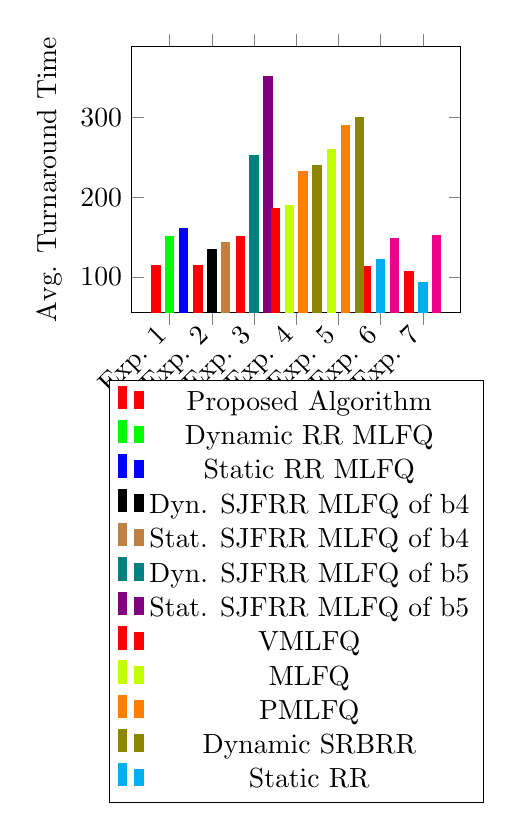
\begin{tikzpicture}
    \begin{axis}[
        width=0.475*\textwidth,
        symbolic x coords={Exp. 1,Exp. 2,Exp. 3,Exp. 4,Exp. 5,Exp. 6,Exp. 7},
        ylabel=Avg. Turnaround Time,
        enlargelimits=0.15,
        legend style={at={(0.5,-0.25)}, anchor=north,legend columns=1},
        ybar,
        xtick={Exp. 1,Exp. 2,Exp. 3,Exp. 4,Exp. 5,Exp. 6,Exp. 7},
        x tick label style={rotate=45,anchor=east},
        bar width=3pt,
        cycle list name=color list
    ]

    \addplot[plot 0,bar group size={0}{3}, red]
    coordinates {(Exp. 1,115) (Exp. 2,115) (Exp. 3,151) (Exp. 6,113.2) (Exp. 7,106.8)};
    \addplot[plot 1,bar group size={1}{3}, green]
    coordinates {(Exp. 1,150.8)};
    \addplot[plot 2,bar group size={2}{3}, blue]
    coordinates {(Exp. 1,161.4)};

    \addplot[plot 1,bar group size={1}{3}, black]
    coordinates {(Exp. 2,134)};
    \addplot[plot 2,bar group size={2}{3}, brown]
    coordinates {(Exp. 2,143.4)};

    \addplot[plot 1,bar group size={1}{3}, teal]
    coordinates {(Exp. 3,252)};
    \addplot[plot 2,bar group size={2}{3}, violet]
    coordinates {(Exp. 3,351)};

    \addplot[plot 0,bar group size={0}{4}, red]
    coordinates {(Exp. 4,185.85) (Exp. 5,212.5)};
    \addplot[plot 1,bar group size={1}{4}, lime]
    coordinates {(Exp. 4,190) (Exp. 5,260)};
    \addplot[plot 2,bar group size={2}{4}, orange]
    coordinates {(Exp. 4,232.14) (Exp. 5,290)};
    \addplot[plot 3,bar group size={3}{4}, olive]
    coordinates {(Exp. 4,240) (Exp. 5,300)};

    \addplot[plot 1,bar group size={1}{3}, cyan]
    coordinates {(Exp. 6,122.4) (Exp. 7,93.6)};
    \addplot[plot 2,bar group size={2}{3}, magenta]
    coordinates {(Exp. 6,148.2) (Exp. 7,152.2)};
    
    \legend{Proposed Algorithm,Dynamic RR MLFQ, Static RR MLFQ, Dyn. SJFRR MLFQ of {b4},  Stat. SJFRR MLFQ of {b4}, Dyn. SJFRR MLFQ of {b5}, Stat. SJFRR MLFQ of {b5}, VMLFQ, MLFQ, PMLFQ, Dynamic SRBRR, Static RR}
    \end{axis}
\end{tikzpicture}
\end{center}
\caption{Comparison graph for average turnaround time}
\vspace{45mm}
\end{figure}

\begin{figure}[H]
    \begin{center}
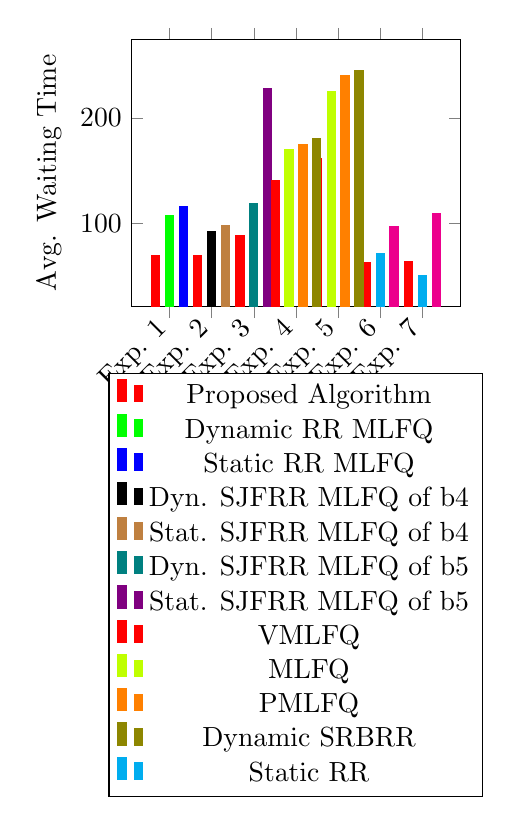
\begin{tikzpicture}
    \begin{axis}[
        width=0.475*\textwidth,
        symbolic x coords={Exp. 1,Exp. 2,Exp. 3,Exp. 4,Exp. 5,Exp. 6,Exp. 7},
        ylabel=Avg. Waiting Time,
        enlargelimits=0.15,
        legend style={at={(0.5,-0.25)}, anchor=north,legend columns=1},
        ybar,
        xtick={Exp. 1,Exp. 2,Exp. 3,Exp. 4,Exp. 5,Exp. 6,Exp. 7},
        x tick label style={rotate=45,anchor=east},
        bar width=3pt,
        cycle list name=color list
    ]

    \addplot[plot 0,bar group size={0}{3}, red]
    coordinates {(Exp. 1,68.8) (Exp. 2,68.8) (Exp. 3,88.7) (Exp. 6,62.4) (Exp. 7,63.4)};
    \addplot[plot 1,bar group size={1}{3}, green]
    coordinates {(Exp. 1,107.6)};
    \addplot[plot 2,bar group size={2}{3}, blue]
    coordinates {(Exp. 1,116.2)};

    \addplot[plot 1,bar group size={1}{3}, black]
    coordinates {(Exp. 2,91.8)};
    \addplot[plot 2,bar group size={2}{3}, brown]
    coordinates {(Exp. 2,98.2)};

    \addplot[plot 1,bar group size={1}{3}, teal]
    coordinates {(Exp. 3,119)};
    \addplot[plot 2,bar group size={2}{3}, violet]
    coordinates {(Exp. 3,228)};

    \addplot[plot 0,bar group size={0}{4}, red]
    coordinates {(Exp. 4,140.14) (Exp. 5,161.75)};
    \addplot[plot 1,bar group size={1}{4}, lime]
    coordinates {(Exp. 4,170) (Exp. 5,225)};
    \addplot[plot 2,bar group size={2}{4}, orange]
    coordinates {(Exp. 4,175) (Exp. 5,240)};
    \addplot[plot 3,bar group size={3}{4}, olive]
    coordinates {(Exp. 4,180) (Exp. 5,245)};

    \addplot[plot 1,bar group size={1}{3}, cyan]
    coordinates {(Exp. 6,71.6) (Exp. 7,50.2)};
    \addplot[plot 2,bar group size={2}{3}, magenta]
    coordinates {(Exp. 6,97.2) (Exp. 7,108.8)};
    
    \legend{Proposed Algorithm,Dynamic RR MLFQ, Static RR MLFQ, Dyn. SJFRR MLFQ of {b4},  Stat. SJFRR MLFQ of {b4}, Dyn. SJFRR MLFQ of {b5}, Stat. SJFRR MLFQ of {b5}, VMLFQ, MLFQ, PMLFQ, Dynamic SRBRR, Static RR}
    \end{axis}
\end{tikzpicture}
\end{center}
\caption{Comparison graph for average waiting time}
\end{figure}

%%%%%%%%%%%%%%%%%%%%%%%%%%%%%%%%%%%%%%%%%%%%%%%%%%%%%%%%%%%%%%%%%%%%%%%%%%%%%%%%%%%
%%%%%%%%%%%%%%%%%%%%%%%%%%%%%%%%%%% CONCLUSION %%%%%%%%%%%%%%%%%%%%%%%%%%%%%%%%%%%%
%%%%%%%%%%%%%%%%%%%%%%%%%%%%%%%%%%%%%%%%%%%%%%%%%%%%%%%%%%%%%%%%%%%%%%%%%%%%%%%%%%%

\section{Conclusion and Future Work}

The goal of this paper is to tackle different shortcomings associated with the standard MLFQ scheduling algorithm as well as its variants discussed in several papers. To resolve these deficiencies, we introduced different adjustable policies and techniques. It is evidently clear that those methods yield better CPU performance and optimize utilization by reducing the average waiting time as well as the average turnaround time. Despite experimenting numerous combinations of the parameters and scheduling policies by which the proposed MLFQ algorithm operates, we can say that there is yet a large room for experiment and improvement through finding better methods and policies which would make the algorithm more adaptable to the nature of the submitted processes and overall more enhanced. For instance, adjusting the criteria by which the schedular decides whether to promote a process might further lessen starvation. Making the proposed algorithm preemptive might also aid mitigating starvation and render overall better performance. The possibilities are limitless.

%%%%%%%%%%%%%%%%%%%%%%%%%%%%%%%%%%%%%%%%%%%%%%%%%%%%%%%%%%%%%%%%%%%%%%%%%%%%%%%%%%%
%%%%%%%%%%%%%%%%%%%%%%%%%%%%%%%%%%%% REFERENCES %%%%%%%%%%%%%%%%%%%%%%%%%%%%%%%%%%%
%%%%%%%%%%%%%%%%%%%%%%%%%%%%%%%%%%%%%%%%%%%%%%%%%%%%%%%%%%%%%%%%%%%%%%%%%%%%%%%%%%%

\begin{thebibliography}{00}

\bibitem{b1} Muhammet Mustafa Ozdal and M. D. F. Wong, "Archer: a history-driven global routing algorithm," \textit{2007 IEEE/ACM International Conference on Computer-Aided Design}, San Jose, CA, 2007, pp. 488-495, doi: 10.1109/ICCAD.2007.4397312.



\end{thebibliography}

\end{document}
